	%------------------------------------------------------------
	%|					CHAPTER 2		                     	|  
	%| PHÂN TÍCH THỰC TRẠNG CỦA VẤN ĐỀ CÓ LIÊN QUAN ĐẾN
    %| ĐỀ TÀI MÀ SINH VIÊN CHỌN VIẾT BÁO CÁO THỰC TẬP TẠI DOANH NGHIỆP THỰC TẬP             			|
	%------------------------------------------------------------
	\pagestyle{fancy}
	\fancyhf{}
	\fancyfoot[R]{\thepage}
\begin{flushleft}
    \fontsize{16}{13}\selectfont
    \section*{CHƯƠNG 2: PHÂN TÍCH THỰC TRẠNG CỦA VẤN ĐỀ CÓ LIÊN QUAN ĐẾN
    ĐỀ TÀI MÀ SINH VIÊN CHỌN VIẾT BÁO CÁO THỰC TẬP TẠI DOANH NGHIỆP THỰC TẬP}
    \addcontentsline{toc}{section}{CHƯƠNG 2: PHÂN TÍCH THỰC TRẠNG CỦA VẤN ĐỀ CÓ LIÊN QUAN ĐẾN
    ĐỀ TÀI MÀ SINH VIÊN CHỌN VIẾT BÁO CÁO THỰC TẬP TẠI DOANH NGHIỆP THỰC TẬP}
    \fontsize{13}{20}\selectfont
    \paragraph{}

    \fontsize{13}{13}\selectfont{Trong thời đại công nghệ 4.0 hiện nay, việc Internet Of Things và AI trở nên bao phủ hầu hết ở mọi mặt của cuộc sống, ngành nghề. Qua nhiều năm, IOT và AI dần chứng minh được chúng có thể thay thế được con người ở rất nhiều lĩnh vực, một số lĩnh vực đạt được phát triển ấn tượng nhờ vào việc ứng dụng IOT và AI tiêu biểu như : y tế, chính trị, kinh doanh, sản xuất. \\ \paragraph{} Việc AI ở thành công nghệ của mọi ngành trở nên thực tế hơn bao giờ hết, ở doanh nghiệp mà em đang tham gia thực tập đặt ra một vấn đề như sau: Phát triển ra một phần mềm có thể hỗ trợ trong việc giám sát từ xa và đưa ra cảnh báo nếu như các chủ thể không ở trong vùng/khu vực được quy định trước đó. Ứng dụng trong thực tế, vấn đề này có thể được đặt khi với các trường hợp như : Giám sát trẻ em, trẻ sơ sinh trong phòng, giám sát công nhân viên trong văn phòng công ty, giám sát hàng hóa trong siêu thị, giám sát các công nhân trong xưởng sản xuất.}
        
    \setcounter{section}{2}
    \setcounter{subsection}{0}
    
    \subsection{Giải Pháp}
    \fontsize{13}{13}\selectfont\paragraph{}
    Hiện nay, công nghệ trí tuệ nhân tạo đã đạt được những thành tựu mang tính lịch sử.Ứng với các giác quan của con người, trí tuệ nhân tạo có thể là bộ não( các phương pháp lí thuận thông minh như : LLM), là đôi mắt ( Thị giác máy tính), là cái miệng ( Text to speech). Trong yêu cầu trên, em đề xuất sử dụng mô hình học sâu để có thể giám sát được các chủ thể và OpenCV để thao tác với các điểm ảnh ( pixel ) trên camera.
    \subsection{Phân tích đánh giá tình hình thực tế theo chủ đề thực tập tại đơn vị}
    \fontsize{13}{13}\selectfont 
    Vấn đề được đặt ra là phải làm sao để có thể xác định được chủ thể con người trong camera (Camera an ninh, điện thoại,...) và xác nhận xem chủ thể có ở trong khu vực được đánh dấu là an toàn hay không, vấn đề này có thể được áp dụng vào các tình huống trong đời sống hàng ngày cũng như trong doanh nghiệp, sản xuất:\\ 
    
    \begin{itemize}
        \item Trong gia đình: \\
        Bài toán này có thể giúp phụ huynh có thể trông con em mình, ví dụ như thông qua camera giám sát và các điểm thiết lập đã được cài đặt sẵn,phụ huynh có thể giám sát được xem là trẻ có đang trong khu vực an toàn hay không,...
        \begin{figure}[htbp]
            \centering
            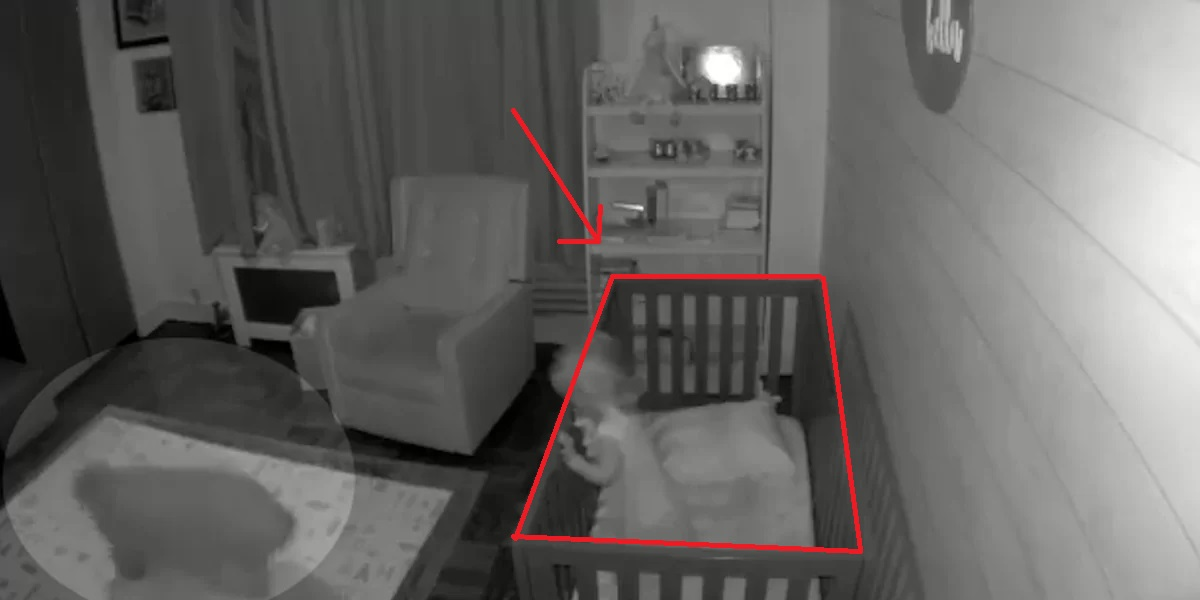
\includegraphics[width=0.5\textwidth]{images/TH1.jpg}
            \caption{Trong trường hợp gia đình.}
            \label{fig:img_1_GD}
        \end{figure}
        \item Trong văn phòng:\\
        Trong văn phòng, có thể giám sát xem, nhân viên có đang làm việc trong khu vực chỉ định hay không,...
        \begin{figure}[htbp]
            \centering
            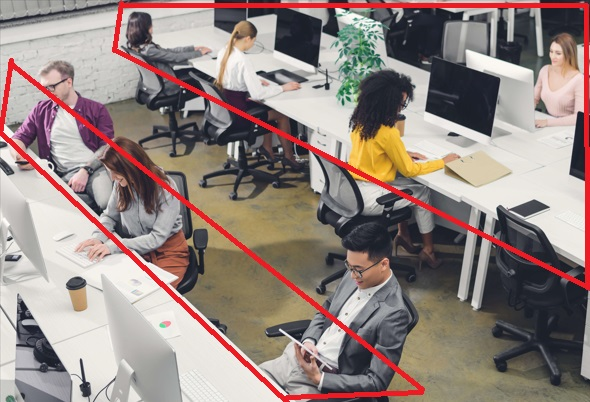
\includegraphics[width=0.5\textwidth]{images/TH2.jpg}
            \caption{Trong trường hợp văn phòng.}
            \label{fig:img_2_VP}
        \end{figure}
        \item Trong sản xuất:\\
        Trong sản xuất, việc các công nhân có làm đúng được vị trí của mình được phân công hay không,...
        \begin{figure}[htbp]
            \centering
            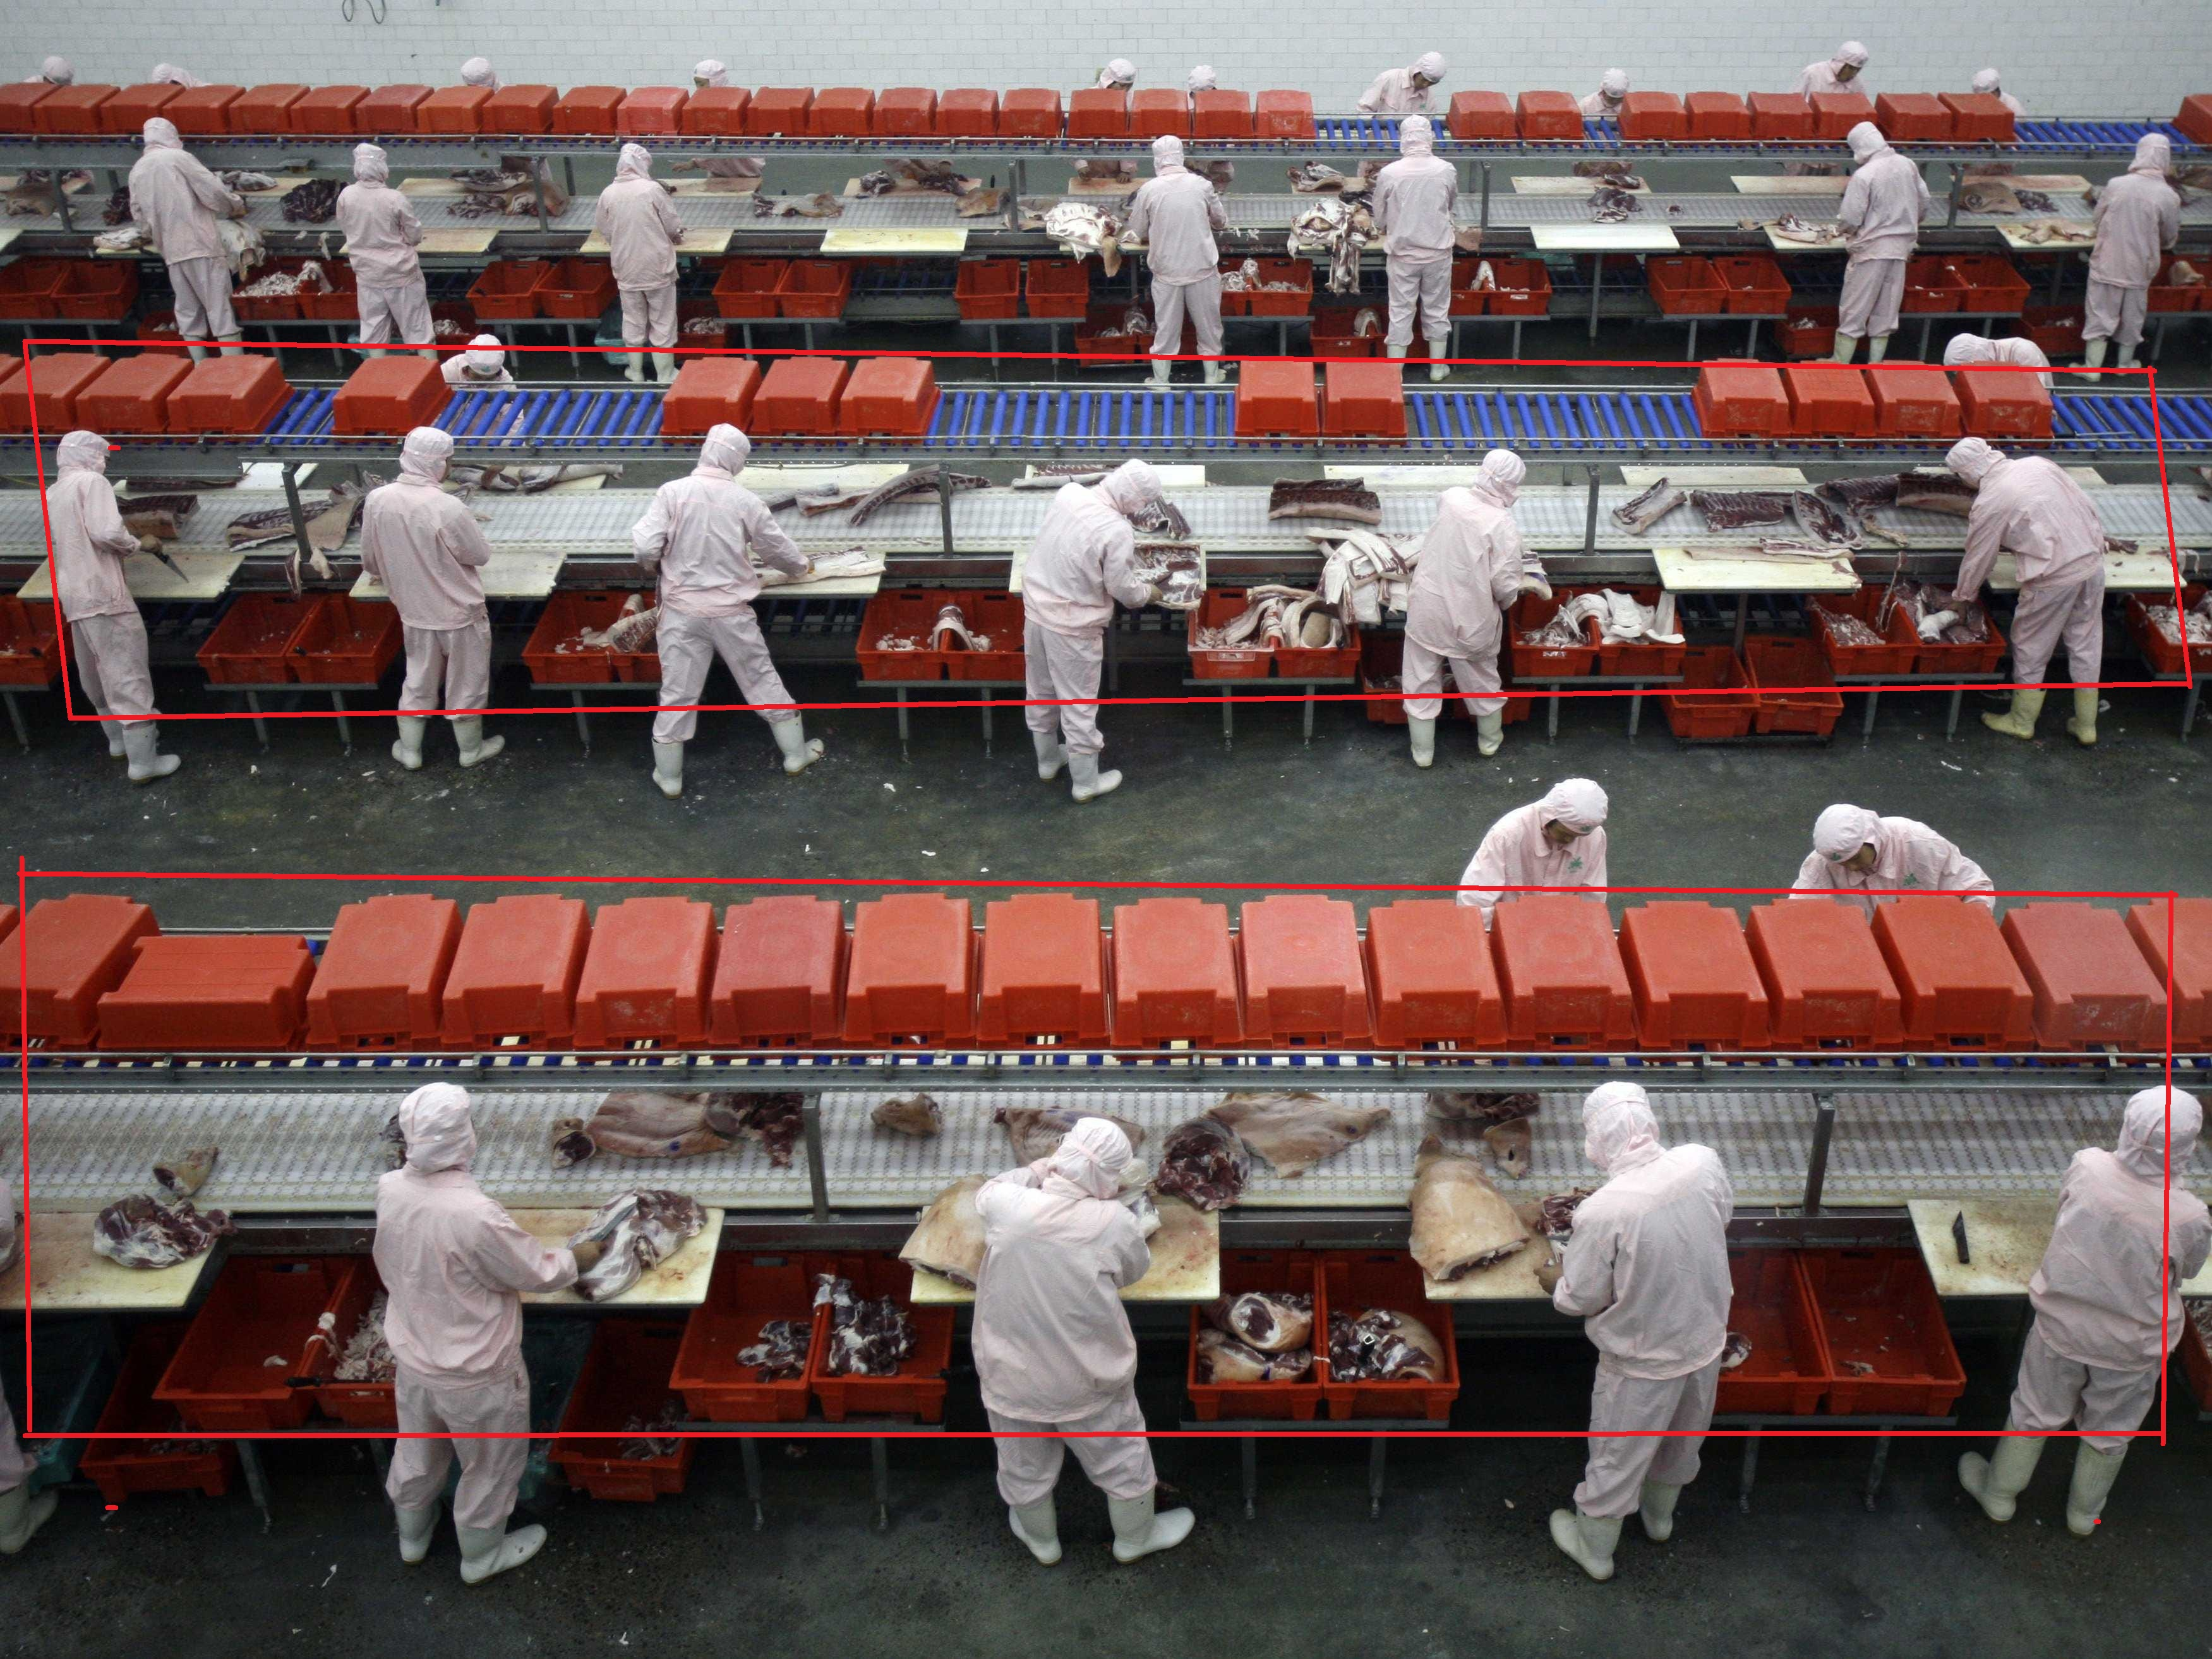
\includegraphics[width=0.5\textwidth]{images/TH3.jpg}
            \caption{Trong trường hợp xí nghiệp.}
            \label{fig:img_3_XN}
        \end{figure}
        \pagebreak
    \end{itemize}
    

    
    \subsection{Ưu điểm, hạn chế của vấn đề phân tích nêu trên}
    \subsubsection{Ưu điểm}
    \fontsize{14}{13}\selectfont\paragraph{}
    Đã thành công trong việc nhận dạng các đối tượng là con người trong ảnh với độ chính xác trung bình khi nhận dạng đối tượng đạt trên 90\%. Có thể giám sát được đối tượng theo thời gian thực nhờ vào công nghệ giám sát học sâu YOLO. Đưa ra các phán đoán dựa trên các khung viền với tốc độ thời gian thật.
    \subsubsection{Hạn chế}
    \fontsize{14}{13}\selectfont\paragraph{}
    Chưa được tối ưu hóa với nhiều thiết bị phần cứng có cấu hình thấp,việc thiết lập sản phẩm phẩn mềm không dễ tiếp cận đối với tập người dùng phổ thông.
    \subsection{Tiến độ thực hiện công việc}
    \begin{tabular}{cp{9cm}}
        \toprule
        Tuần thực hiện & Nội dung thực hiện \\
        \midrule
        Tuần 1    & Làm quen với công ty và các đồng nghiệp, thiết lập môi trường làm việc 
                    và các phần mềm cần thiết cho công việc tại công ty. \\
        \addlinespace
        Tuần 2    & Nhận yêu cầu từ người hướng dẫn, lên kế hoạch và chọn ra các công nghệ phù hợp với yêu cầu của vấn đề. \\
        \addlinespace
        Tuần 3-5    & Bắt tay vào làm và học hỏi từ các bản mẫu, các tài liệu chuyên ngành. Thử nghiệm trên phần cứng và cho ra được bản mẫu cơ bản. \\
        \addlinespace
        Tuần 6-9    & Chỉnh sửa, cải tiến liên tục để có thể tương thích với các trường hợp được đặt ra cho phù hợp với tình hình thực tế của yêu cầu. \\
        \addlinespace
        Tuần 10    & Viết các file thông số và cài đặt với sản phẩm. \\
        \addlinespace
        Tuần 11-16    & Tổng hợp lại quá trình làm, viết các báo cáo, thu hoạch và kết thúc thực tập.\\
        \bottomrule
      \end{tabular}
    \subsection{Sơ lược các kỹ thuật, công nghệ liên quan đến các nội dung đã trình bày}
\end{flushleft}